% thesis.tex
%
% Copyright 2022 Alexander Lyttle.
%
% This work may be distributed and/or modified under the conditions of the
% LaTeX Project Public License (LPPL) version 1.3 or later.
%
% The latest version of this license is in
% https://www.latex-project.org/lppl.txt and version 1.3 or later is part of
% all distributions of LaTeX version 2005/12/01 or later.
%
% This work consists of the files uobthesis.cls, packages.sty, and thesis.tex.
%
%
%% PREAMBLE ===================================================================
%
% UoB recommends A4 paper and a font size of 12pt
\documentclass[a4paper,12pt]{uobthesis}


%% PACKAGES -------------------------------------------------------------------
%
% Packages and setup are in packages.sty
\usepackage{packages}

% Add any additional packages below or at the bottom of packages.sty


%% RESOURCES ------------------------------------------------------------------
%
% Add bibliography resource files
\addbibresource{references.bib}

% Add glossary files
% === GLOSSARY OF ACRONYMS ===
%
% For the list of acronyms to appear, you need to:
% pdflatex thesis.tex
% makeglossaries thesis
% pdflatex thesis.tex
%
% List your acronyms here, e.g.
\newacronym{ms}{MS}{main sequence}

% === GLOSSARY OF TERMS ===
%
% For the list of terms to appear, you need to:
% pdflatex thesis.tex
% makeglossaries thesis
% pdflatex thesis.tex
%
% List of terms go here, e.g.
\newglossaryentry{luminosity}
{
    name=luminosity,
    description={The total radiant power of an object}
}
\newglossaryentry{star}
{
    name=star,
    description={An astronomical object which is in hydrostatic equilibrium and emits light due to internal sources of energy}
}



%% TITLEPAGE DETAILS ----------------------------------------------------------
%
% Add your details here
\author{Author Name}
\title{Thesis Title}
\group{Your Research Group}
\school{Your School}
\college{Your College}
\submitted{March}{2022}  % Change this to the month you submit your thesis

% Path to UoB logo file, download from 
% https://intranet.birmingham.ac.uk/staff/resources/brand-resources/university-logo-guidelines.aspx
\logo{uob-logo.eps}  % Optional, comment this out if logo not wanted


%% DEDICATION -----------------------------------------------------------------
%
% Optional dedication, edit this or comment out if not appropriate
\dedication{Dedicated to my family.}


%% ABSTRACT -------------------------------------------------------------------
%
\abstract{\lipsum[1-2]}


%% ACKNOWLEDGEMENTS -----------------------------------------------------------
%
\acknowledgements{\lipsum[3-6]}


%% DOCUMENT ===================================================================
%
\begin{document}

  \maketitle  % Title page

  \frontmatter

  %% FRONT MATTER -------------------------------------------------------------
  \makefrontmatter  % Adds abstract, dedication and acknowledgements

  %% CONTENTS -----------------------------------------------------------------
  \tableofcontents
  \listoffigures
  \listoftables
  \printglossary[type=\acronymtype,title={List of Acronyms}]
  \printglossary[title={List of Terms}]

  \mainmatter

  %% CHAPTERS -----------------------------------------------------------------
  %
  % Add your chapters here
  % chapters/introduction.tex
%
% Copyright 2022 Alexander Lyttle.
%
% This work may be distributed and/or modified under the conditions of the
% LaTeX Project Public License (LPPL) version 1.3 or later.
%
% The latest version of this license is in
% https://www.latex-project.org/lppl.txt and version 1.3 or later is part of
% all distributions of LaTeX version 2005/12/01 or later.
%
%
\chapter{Introduction}

\lipsum[7-12]
  % chapters/example.tex
%
% Copyright 2022 Alexander Lyttle.
%
% This work may be distributed and/or modified under the conditions of the
% LaTeX Project Public License (LPPL) version 1.3 or later.
%
% The latest version of this license is in
% https://www.latex-project.org/lppl.txt and version 1.3 or later is part of
% all distributions of LaTeX version 2005/12/01 or later.
%
%
\chapter{Example Chapter}

This chapter covers some basic usage of the packages bundled with this template.

\section{Citations and References}

This template uses \texttt{biblatex} to produce the bibliography. The citation style for this template is author-year and it uses \texttt{natbib} to provide in-text and parenthesis citation styles with additional commands \texttt{citep} and \texttt{citet}. Go to \texttt{packages.sty} to customise these options to suit your preferred citation style. Otherwise, here are some examples for the chosen style in this template. Here is an example citation in parentheses \citep{einstein} or we can just refer to \citet{dirac} in text. Notice that just using the basic \texttt{cite} command produces the same as \texttt{citep} without parentheses, \cite{knuth-fa}. Citations in parenthesis can have info before and after \citep[e.g.][chap. 2]{dirac}. You can cite multiple sources in parentheses \citep{einstein,knuth-fa,dirac} or in text \citet{einstein,dirac,knuth-fa}. Notice that they are put into ascending date order.

Use the \texttt{href} package to create external links, but be aware that this won't translate well in print. For example, see the GitHub repository for this template \href{https://github.com/alexlyttle/uob-thesis-template}{here}. To make the reference print-friendly, you could put the full address in text with the \texttt{url} command (\url{https://github.com/alexlyttle/uob-thesis-template}) or in a footnote\footnote{\url{https://github.com/alexlyttle/uob-thesis-template}}.

\section{Glossary Usage}

This template uses the \texttt{glossaries} package. Each glossary item should be defined in the document preamble. Here, these are separated into the files \texttt{glossary/acronyms.tex} and \texttt{glossary/terms.tex} for your convenience. To refer to glossary items, there are several commands. For example, \texttt{\textbackslash gls\{<term\_name>\}} will reference the glossary item for \texttt{<term\_name>}. Acronyms should first be referenced with \texttt{\textbackslash acrfull\{ms\}} and subsequently with \texttt{\textbackslash acrshort\{ms\}}. Some example usage is given in Section \ref{sec:figandtab}.

\section{Quantities and Units}

Quantities and their units can be formatted consistently with the \texttt{siunitx} package. This can be configured in \texttt{packages.sty}. For example, large numbers are formatted like this, \num{123456789}. Quantities with units are formatted like this, \SI{50}{\meter\per\second\squared}, and can be used in math mode $\nu = \SI{8}{\micro\hertz}$. Uncertainties can be included using the parentheses shorthand, \SI{102(3)}{\meter\per\second}. Units can be given on their own, for example \si{\centi\meter}. Custom units may also be defined in the preamble. The SI unit formats may be configured with the \texttt{\textbackslash sisetup} command.

\section{Figures and Tables}\label{sec:figandtab}

\Glspl{star} spend most of their life on the \acrfull{ms}. The \acrshort{ms} was discovered when the \gls{luminosity} of many stars were plot against their spectral class. We can see this in Figure \ref{fig:example}. For good print quality, figures should be produced with at least 300 \acrfull{dpi}. To consistently achieve this, avoid resizing your images and produce them to this specification. Using A4 paper size with the default document class margins, the text width is \SI{160}{\milli\meter}.

\begin{figure}[t]
  \centering
  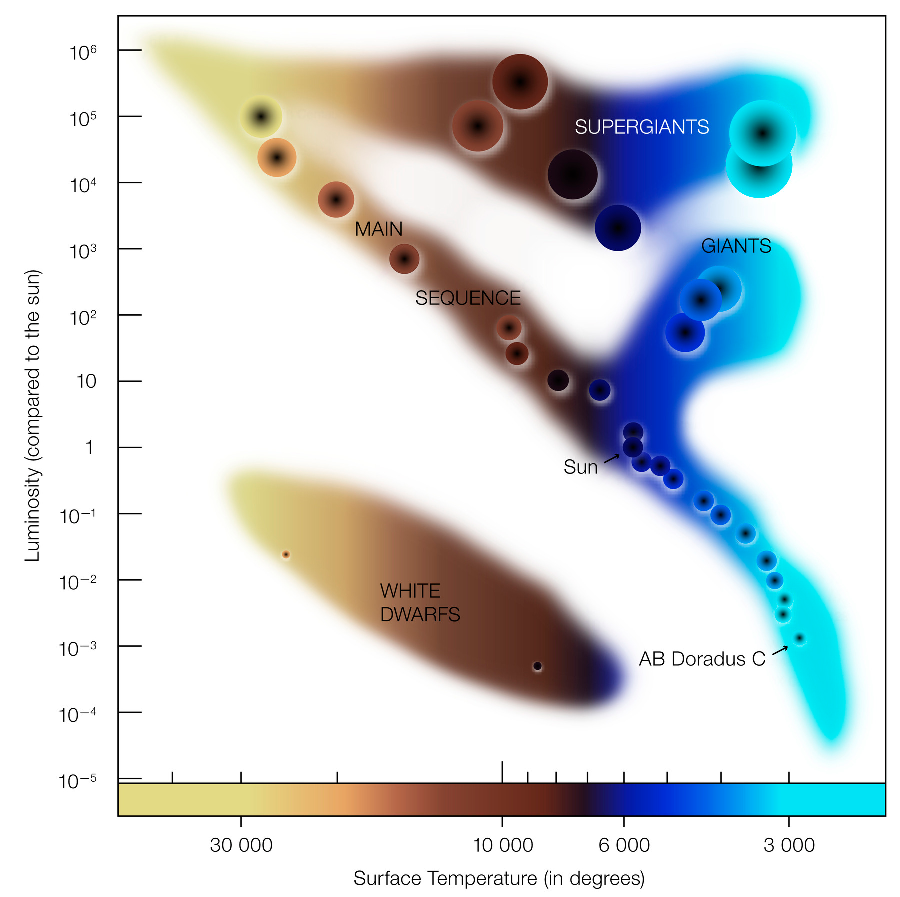
\includegraphics{figures/example.pdf}
  \caption[Short version of caption]{The Hertzsprung-Russell diagram produced by the European Southern Observatory. \emph{Credit:} \href{https://www.eso.org/public/images/eso0728c/}{ESO}.}
  \label{fig:example}
\end{figure}

Table \ref{tab:example} is completely unrelated to Figure \ref{fig:example} but we have thrown that in as another example. The table requires the \texttt{booktabs} package. This template stores figures and tables in separate folders. For your own sanity, consider keeping tables in separate files for your project. This makes them easy to update with new data.

\begin{table}
  \centering
  \caption[Short version of caption]{Table caption.}
  \label{tab:example}
  % tables/example.tex
%
% Copyright 2022 Alexander Lyttle.
%
% This work may be distributed and/or modified under the conditions of the
% LaTeX Project Public License (LPPL) version 1.3 or later.
%
% The latest version of this license is in
% https://www.latex-project.org/lppl.txt and version 1.3 or later is part of
% all distributions of LaTeX version 2005/12/01 or later.
%
%
\begin{tabular}{lrrrr}
  \toprule
  Name & A & B & C & D \\
  \midrule
  One & 1 & 2 & 3 & 4 \\
  \bottomrule
\end{tabular}

\end{table}

\section{Equations}

Here are some example equations making use of the \texttt{amsmath} and \texttt{bm} packages. An example single line equation,
%
\begin{equation}
  f(x) = - \frac{2}{x^3},\label{eq:func}
\end{equation}
%
can be referenced to as Equation \ref{eq:func}. 

A multi-line equation,
%
\begin{align}
  y &= \int f(x) \mathrm{d} x,\label{eq:int}\\
  &= \frac{1}{x^2},\label{eq:sol}
\end{align}
%
can be referenced to as Equations \ref{eq:int} and \ref{eq:sol}.

Also, here is a vector written in an unnumbered equation,
%
\begin{equation*}
  \vec{a} \equiv \bm{a} = 
  \begin{bmatrix}
    x\\y\\z
  \end{bmatrix}
  ,
\end{equation*}
%
where the \texttt{bmatrix} environment is used to format the column vector.

  
  %% BIBLIOGRAPHY -------------------------------------------------------------
  %
  \printbibliography[title=References,heading=bibintoc]

  %% APENDICES ----------------------------------------------------------------
  %
  \appendix

  % Add your appendices here
  % appendices/example.tex
%
% Copyright 2022 Alexander Lyttle.
%
% This work may be distributed and/or modified under the conditions of the
% LaTeX Project Public License (LPPL) version 1.3 or later.
%
% The latest version of this license is in
% https://www.latex-project.org/lppl.txt and version 1.3 or later is part of
% all distributions of LaTeX version 2005/12/01 or later.
%
%
\chapter{Example Appendix}

\lipsum[25-30]


\end{document}
